\documentclass[conference]{IEEEtran}
\IEEEoverridecommandlockouts
% The preceding line is only needed to identify funding in the first footnote. If that is unneeded, please comment it out.
\usepackage{cite}
\usepackage{textcomp}
\usepackage[dvipsnames, table]{xcolor}


\usepackage{booktabs,multirow,array,hhline}
\newcolumntype{N}{@{}m{0pt}@{}}
%\usepackage[margin=15mm]{geometry}
\usepackage{amsmath}
\usepackage{amssymb}
\usepackage{bm}
\usepackage{amsfonts}
\usepackage{tikz}
\usepackage{mathdots}
\usepackage{cancel}
\usepackage{color}
\usepackage{siunitx}
\usepackage{array}
\usepackage{multirow}
\usepackage{gensymb}
\usepackage{tabularx}
\usepackage{booktabs}
\usetikzlibrary{fadings}
\usetikzlibrary{patterns}
\usetikzlibrary{shadows.blur}
\usepackage{booktabs} % For formal tables
\usepackage{graphicx}
\usepackage{mathtools}
\usepackage{subcaption}
\usepackage{xspace}
% \captionsetup{compatibility=false}
\usepackage[ruled,vlined, linesnumbered]{algorithm2e}
\usepackage{import}
\usepackage{url}

% table and siunits
\usepackage{tabularx, siunitx}
\newcommand{\best}{{\cellcolor[gray]{0.75}}}
\newcommand{\statsimilar}{{\cellcolor[gray]{0.9}}}
\newcommand{\algremark}[1]{\tcc*[r]{#1}}
\newcommand{\iqr}{{\small}}

\usepackage[noend]{algpseudocode}
\makeatletter
\def\BState{\State\hskip-\ALG@thistlm}
\makeatother


%% MATHS COMMANDS
% for algorithms
\DeclarePairedDelimiter\abs{\lvert}{\rvert}%
\DeclareMathOperator*{\evaluatedx}{\bX}
\DeclareMathOperator*{\paretofront}{\mathcal{P}}
\DeclareMathOperator*{\paretoset}{\evaluatedx_{\mathcal{P}}}
\DeclareMathOperator*{\attainmentfront}{\mathcal{A}}
\DeclareMathOperator*{\attainmentset}{\evaluatedx_{\mathcal{A}}}
\DeclareMathOperator*{\ninitialevaluations}{N}
\DeclareMathOperator*{\nevaluations}{m}
\DeclareMathOperator*{\nbudget}{B}
\DeclareMathOperator*{\parameterspace}{\Omega}
\DeclareMathOperator*{\ndim}{d}
\DeclareMathOperator*{\nobj}{M}
\DeclareMathOperator*{\rp}{\mathbf{R}}


\DeclareMathOperator*{\sig}{sig}
\DeclareMathOperator*{\saf}{SAF}
\DeclareMathOperator*{\msafmu}{SAF_\mu}
\DeclareMathOperator*{\OSAF}{osaf}
\DeclareMathOperator*{\DSAF}{dsaf}
\DeclareMathOperator*{\MMIN}{maximin}
\DeclareMathOperator*{\MMAX}{minimax}
\DeclareMathOperator*{\mgp}{\mathcal{GP}}


\DeclareMathOperator*{\union}{\medcup}
\DeclareMathOperator*{\argmax}{\arg\!\max}
\DeclareMathOperator*{\argmin}{\arg\!\min}
\DeclareMathOperator*{\bigO}{\mathcal{O}}
\DeclareMathOperator*{\erf}{\text{erf}}
\DeclareMathOperator*{\cov}{\text{cov}}
\DeclareMathOperator{\diag}{diag}
\DeclareMathOperator{\nondom}{nondom}
\DeclareMathOperator{\LatinHypercubeSampling}{LHS}
\DeclareMathOperator{\posterioruncertainty}{\bm{\sigma}}


\DeclareMathOperator*{\igdp}{IGD^{+}}




\newcommand\safmu{SAF$_{\mu}$\xspace}
\newcommand\safei{SAF$_{EI}$\xspace}
\newcommand\smsego{SMS-EGO\xspace}
\newcommand\smsegomu{SMS-EGO$_{\mu}$\xspace}
\newcommand\parego{ParEGO\xspace}
\newcommand\mpoi{MPoI\xspace}
\newcommand\ei{EI\xspace}
\newcommand\gp{GP\xspace}
\newcommand\gps{GPs\xspace}
\newcommand\maximin{maximin\xspace}
\newcommand\lhs{LHS\xspace}
\newcommand\igd{IGD$^+$\xspace}

\newcommand\target{\mathcal{T}}
\newcommand\mF{\mathcal{F}}
\newcommand\mP{\mathcal{P}}
\newcommand\Papprox{\tilde{\mathcal{P}}}
\newcommand\mGP{\ensuremath{\mathcal{GP}}\xspace}
\newcommand\mD{\mathcal{D}}
\newcommand\mN{\mathcal{N}}
\newcommand\mX{\mathcal{X}}
\newcommand\normal{\mathcal{N}}
\newcommand{\inv}{^{-1}}
\newcommand\natnum{\mathbb{N}}
\newcommand\expc{\mathbb{E}}
\newcommand*{\medcup}{\mathbin{\scalebox{1.5}{\ensuremath{\cup}}}}

\newcommand{\trp}{^\top}
\newcommand{\given}{\,|\,}



\newcommand{\pigdref}{\mathcal{Z}}
\newcommand{\bx}{\mathbf{x}}
\newcommand{\bX}{\mathbf{X}}
\newcommand{\by}{\mathbf{y}}
\newcommand{\bI}{\mathbf{I}}
\newcommand{\bz}{\mathbf{z}}
\newcommand{\brr}{\mathbf{r}}
\newcommand{\bff}{\mathbf{f}}
\newcommand{\bF}{\mathbf{F}}
\newcommand{\bzero}{\mathbf{0}}
\newcommand{\bmu}{\boldsymbol{\mu}}
\newcommand{\bphi}{\boldsymbol{\phi}}
\newcommand{\fhat}{\hat{f}}
\newcommand{\fstar}{f^\star}
\newcommand{\xnext}{\bx'}
\newcommand{\data}{\mathcal{D}}
\newcommand{\FIXME}[1]{[\textcolor{red}{\textbf{FIXME} \textsl{#1}]}}
\newcommand{\mnote}[2][\textcolor{red}{\dagger}]{$#1$\marginpar{\color{red}\raggedright\tiny$#1$
    #2}}
\newcommand{\fnote}[2][\textcolor{teal}{\dagger}]{$#1$\marginpar{\color{teal}\raggedright\tiny$#1$
    #2}}
    

\newcommand*{\eg}{e.g.\@\xspace}
\newcommand*{\ie}{i.e.\@\xspace}
\newcommand*{\etal}{\textit{et al.}\@\xspace}

\begin{document}

%
\title{Multi-objective Bayesian optimisation using an exploitative summary attainment front acquisition function}

%Exploitative and Bayesian multi-objective optimisation: a summary attainment front acquisition function
%

\author{
  \IEEEauthorblockN{Finley J. Gibson}
  \IEEEauthorblockA{\textit{Department of Computer Science,}\\
      \textit{University of Exeter,}\\
      Exeter, UK\\
      \url{F.J.Gibson@exeter.ac.uk}
      }
      \and
       \IEEEauthorblockN{Richard M. Everson}
  \IEEEauthorblockA{\textit{Department of Computer Science,}\\
      \textit{University of Exeter,}\\
      Exeter, UK\\
      \url{R.M.Everson@exeter.ac.uk}
      }
      \and
       \IEEEauthorblockN{Jonathan E. Fieldsend}
       \IEEEauthorblockA{\textit{Department of Computer Science,}\\
      \textit{University of Exeter,}\\
      Exeter, UK\\
      \url{J.E.Fieldsend@exeter.ac.uk}
    }
  }

  \maketitle

\begin{abstract}

    %Efficient methods for optimising expensive black-box problems with multiple objectives can often themselves become prohibitively expensive as the number of objectives is increased. We propose an approach to efficient optimisation of such problems without the reliance on hypervolume and expected improvement computation, which are the principal causes of poor dimensional scaling in current state-of-the-art  approaches.  We show that our approach is able deliver similar performance to the current state-of-the-art, and further show that approaches based on surrogate mean predictions are superior to the widely used \textit{expected improvement} when\mnote{with?} the Gaussian process surrogate models, typically applied. Performance is evaluated on the well-known Walking Fish Group problem set, against current state-of-the art approaches. 
 
    Efficient methods for optimising expensive black-box problems with multiple objectives can often themselves become prohibitively expensive as the number of objectives is increased. We propose an infill criterion based on the distance to the summary attainment front which does not rely on the expensive hypervolume or expected improvement computations, which are the principal causes of poor dimensional scaling in current state-of-the-art approaches. By evaluating performance on the well-known Walking Fish Group problem set, against current state-of-the art approaches, we show that our method  delivers similar performance to the current state-of-the-art.  We further show that methods based on surrogate mean predictions are more often than not superior to the widely used expected improvement, suggesting that the additional exploration produced by accounting for the uncertainty in the surrogate's prediction of the optimisation landscape is often unnecessary and does not aid convergence towards the Pareto front. 

\end{abstract}


\begin{IEEEkeywords}
Expensive optimisation, Bayesian optimisation, infill criteria, acquisition functions.
\end{IEEEkeywords}


\section{Introduction}
The process of optimising black-box functions relies exclusively on querying the underlying objective function in order to advance the understanding of the parameter objective-space mapping of, and convergence toward, an optimal solution. During the optimisation process a balance must be struck between the exploitation of the function as currently understood in order to find good solutions, and further exploration of the unknown regions of its landscape in order to advance this understanding. Extensive work has gone into theorising how this balance should be managed, particularly in cases where there is a high cost associated with querying the underlying objective. In such cases careful management of this balance is considered essential if a suitable solution is to be found as efficiently as possible. Bayesian optimisation \cite{jones1998efficient} has emerged as an effective means of solving such problems, and has been widely applied to many problems with success.

In the field of multi-objective optimisation (MO), efforts have been made to employ similar strategies to those used for single objective optimisation, but accurately modelling the multi-dimensional objective space is more challenging, and many techniques used in single-objective optimisation require complex volume measurement and integration, the computational complexity of which scales poorly in the higher dimensional objective spaces associated with MO. One widely used technique is the computation of the expected improvement (\ei) to manage the exploitation/exploration trade-off. However, recent work has shown that in single objective problems with high-dimensional parameter spaces, the low fidelity between the commonly used surrogate models and the underlying function reduces the need to actively explore the function. Instead purely exploitative methods have been demonstrated to outperform methods which balance the explore/exploit trade-off, when the fidelity between the surrogate and true function is low \cite{death2019greed}. With this in mind we look apply to this exploitative approach to the multi-objective domain, where we believe the increased complexity of modelling problems with multi-dimensional outputs will enjoy similar benefits of an exploitative approach. 

In this paper we address a particular set of mutli-objective problems (MOPs), for which some cost associated with the evaluation of the objectives for a set of parameters is significant, and restricts the number of queries of the objective function can be made. This can be because either each objective is independently expensive and requires a separate evaluation or, more commonly, all objectives are jointly evaluated by a single expensive process. In such MOPs the goal of the optimisation process is to find a suitable solution in as few evaluations of the objective function(s) as possible. The advent of large-scale simulation, and optimisation problems that require physical experimentation to evaluate an objective function has brought this class of Efficient multi-objective optimisation problems (EMOPs) to the fore as an important area of research. This class of problem is common in real-world applications, particularly in the fields of engineering and computer modelling. For example, when engineering a component based on some design parameters, performance evaluation of a newly proposed design may require making and testing the component, incurring both time and material costs \cite{fang2017design}. Alternately, computationally expensive processes such as fluid dynamic simulation or machine learning model evaluation, often have high computational costs associated with them and can take hours or even days to process \cite{huband2005scalable}. This renders optimiser classes such as Multi-Objective Evolutionary Algorithms\cite{tanabe2017benchmarking,coello2007evolutionary} or Multi-Objective Genetic Algorithms\cite{tamaki1996multi}, for which a large number of objective evaluations are required, unsuitable. 

\section{Background}
\subsection{Bayesian Optimisation}\label{section:background_BayesianOptimisation}
Bayesian optimisation (BO) is a form of efficient global optimisation (EGO), which searches for the global optimal solution to an objective function $f(\mathbf{x})$ for  $f: \parameterspace \subset \mathbb{R}^{\ndim} \mapsto \mathbb{R}$, while making as few evaluations of the objective function as possible. In BO, in order to limit the number of evaluations required of the true objective function,  a small number of $\ninitialevaluations$ initial evaluations are made, and a probabilistic surrogate model is then generated from these evaluations. This surrogate model, which should be cheap to evaluate, can then be used to predict the efficacy of subsequent candidate solutions without the need to frequently evaluate $f$. 

\begin{algorithm}[t]
  \SetAlgoLined
  \KwResult{minimiser of $f(\bx)$}
  \SetKwInOut{Input}{Input}
  \SetKwInOut{Output}{Output}
  \SetKwComment{tcc}{}{}
  \SetCommentSty{textit}
  \DontPrintSemicolon
  \Input{$\ninitialevaluations$ - number of initial evaluations}
  \Input{$\nbudget$ - evaluation budget}
  \BlankLine
  %\textbf{Initialization}
  %\tcc*[l]{\textbf{Initialisation:}\hfill Generate initial samples}
  $X \gets \text{LHS}(\parameterspace, \ninitialevaluations)$ \label{alg: BO_LHS}
  \algremark{Generate initial samples}
  \For {$t = 1 \xrightarrow{} \ninitialevaluations$ \do}{ \label{alg:initial-start}
    $f_t \gets f(\bx_t)$ \algremark{Expensively evaluate initial samples}
    } \label{alg:initial-end}
  $\data  \gets \{(\bx_t, f_t)\}_{t=1}^{\ninitialevaluations}$
  \BlankLine 

  \For{$t = \ninitialevaluations+1\xrightarrow{}\nbudget$ \do}{
  $ \theta \gets \text{train} \;\mathcal{GP}(\data)$ \label{alg:train}\\
  $\bx_t \gets \underset{\mathbf{x}\in \parameterspace}{\argmax} \:
  \alpha(\mathbf{x}; \theta)$ \label{alg:opt-alpha} \algremark{Maximise acquisition function}
  $ f_t \gets f(\bx_t)$ \label{alg:expensive} \algremark{Expensively evaluate $\bx_t$}
  $\data \gets \data \cup \{(\bx_t, f_t)\}$ \algremark{Augment data}}
  \Output{$\bx_t \quad \quad \underset{t\in 1:\nbudget}{\argmin} f_{1:\nbudget}$}
\caption{Bayesian optimisation}
\label{alg:BO}
\end{algorithm}

The process of BO, summarised in Algorithm \ref{alg:BO}, involves first selecting a set of $\ninitialevaluations$ initial candidate solutions, usually via Latin hypercube sampling (LHS) \cite{mckay2000comparison}, and evaluating the objective function for each of these to produce a set $\mathcal{D} = \{ (\bx_t, f_t \triangleq f(\bx_t) )\}_{t=1}^{\ninitialevaluations}$; lines \ref{alg:initial-start}-\ref{alg:initial-end} in Algorithm \ref{alg:BO}. A probabilistic, surrogate model is then fitted to these observations, for which  Gaussian processes (\gp) are commonly used; see \cite{rasmussen2003gaussian} for a comprehensive introduction.
The \gp describes the current belief about the form of the objective function, modelling it as a set of random variables with a joint Gaussian distribution, and the predictive probability distribution of $\hat{f}(\bx)$ at a location $\bx$ is a normal distribution:
\begin{equation}\label{eqn: P(f_t+1)}
P\big(\hat{f}(\mathbf{x}) \given \mathbf{x}, \mathcal{D}, \theta \big) = 
\mathcal{N}\big(\bmu(\mathbf{x}), \sigma^2(\mathbf{x})\bI\big)
\end{equation}
where
\begin{align}\label{eqn: mu}
\bmu(\mathbf{x}) &= \boldsymbol{\kappa}(\mathbf{x}, \evaluatedx) - K^{-1}  \bphi,\\
\label{eqn: sigma}
\sigma^2(\mathbf{x}) &= \kappa(\mathbf{x}, \mathbf{x}) - \boldsymbol{\kappa}(\mathbf{x}, \evaluatedx)^{\top}K^{-1} \boldsymbol{\kappa}(\evaluatedx, \mathbf{x}).
\end{align}
Where $\evaluatedx$ is the $\ndim$ by $\nevaluations$ matrix of locations at which $f(\bx)$ has
been previously evaluated, $\bphi = (\bx_1, \bx_2, \ldots, \bx_{\nevaluations})$\fnote{check $\nevaluations$ correct here?}.
$\kappa(\mathbf{x}, \mathbf{x}')$ is a predefined
covariance function, or  \textit{kernel}, between $\mathbf{x}$ and
$\mathbf{x}'$, and  $K$ is the covariance matrix comprised of all
covariances $\kappa(\mathbf{x}, \mathbf{x}') \; \forall \: \mathbf{x},
\mathbf{x}'\in \evaluatedx$. A vector of the covariances between
$\mathbf{x}$ and each of the $M$ locations in $\evaluatedx$ is denoted
$\boldsymbol{\kappa}(\mathbf{x}, \evaluatedx)\in \mathbb{R}^{M}$ and
similarly the vector of covariances between each of the $M$ locations in
$\evaluatedx$ and $\mathbf{x}$ is denoted $\boldsymbol{\kappa}(\evaluatedx,
\mathbf{x}) \in \mathbb{R}^{M}$. The parameters of the covariance function
(and any noise model) are denoted by $\theta$, and these are learned on receipt of each new $(\bx, f(\bx))$ pair by maximising the likelihood of the data \cite{rasmussen2003gaussian}; Algorithm \ref{alg:BO} line \ref{alg:train}. 


Determination of how desirable a new evaluation of the objective function
would be at a new location is achieved through application of an acquisition function $\alpha(\mathbf{x};  \theta)$, which balances the exploitation of locations predicted by the surrogate (with parameters $\theta$) to be good with high confidence, with the exploration of regions that have high uncertainty and might therefore contain the optimum. Maximisation of the acquisition function (Algorithm \ref{alg:BO} line \ref{alg:opt-alpha}) yields the next location $\bx'$ at which to evaluate the real objective function: 
\begin{equation}\label{eqn: argmax_alpha}
   \bx' = \underset{\mathbf{x} \in \Omega}{\argmax}\:\alpha(\mathbf{x};  \theta).
\end{equation}
The acquisition function can be cheaply optimised using methods such as an evolutionary algorithm without the need for repeated evaluation of the expensive objective function. Several broadly applicable acquisition functions have been specified, typically based on expected improvement or probability of improvement  measures \cite{jones1998efficient,shahriari2015taking} and \ei has been shown to converge at a near optimal rate \cite{bull2011convergence}. This process of fitting a surrogate, and optimisation of the acquisition function is repeated,  to expand $\mathcal{D}$, iteratively until a good solution is found and some stopping criteria is satisfied or the computational budget is exhausted.

\subsection{Multi-objective Bayesian Optimisation}\label{section:background_MOPs}
In MOPs there is not one single criterion by which the success of a solution is assessed, but rather a series of conflicting objectives, between which some compromise must be reached. We denote the $\nobj$ conflicting objective functions by $f_i(\bx)$, $i = 1, \ldots, \nobj$, so that the MOP may be expressed 
as 
\begin{equation}\label{eqn: min_F}
\underset{\mathbf{x} \in \mX}{\argmin}\:\mathbf{f}(\mathbf{x}), 
\end{equation}
where $\parameterspace \subset \mathbb{R}^n$ is the feasible space and and $\mathbf{f}: \Omega \mapsto \mathbb{R}^{D}$.

A solution $\bx$ is said to dominate another $\bx'$ (denoted $\bx \prec \bx'$) if $f_i(\bx) \le f_i(\bx')$ for $i = 1, \ldots, D$ and $ f_i(\bx) < f_i(\bx')$ for at least one $i$. Since in most cases with conflicting objectives there is no single dominating solution, the goal of most multi-objective optimisation algorithms is to produce a number of solutions which well represent the Pareto set, that is the maximal set of solutions that are not dominated by any other solutions in the feasible space:
\begin{equation}\label{eqn: Pareto_set}
  \paretoset = \{\mathbf{x} \in \parameterspace \;:\;
  \bx' \not\prec \bx \,\forall \bx' \in \parameterspace \}.
\end{equation}
%This is referred to as the summary attainment front (SAF),\mnote{no it is not -- you are confusing spaces and constructs here} and t
The image of $\paretoset$ under $\bff$ is the Pareto front ($\paretofront$). Typically in multi-objective optimisation the best we can aspire to is an \emph{approximation} this, as represented by a set of mutually non-dominating solutions. The $\nobj-1$ dimensional surface in objective space which separates the area/volume dominated by any element of this set from that which is non-dominated is known as the summary attainment front (SAF), hereby denoted $\attainmentfront$, and its parameters $\attainmentset$.
\begin{equation}\label{eqn: Attainment_set}
  \attainmentset = \{\mathbf{x} \in \evaluatedx \;:\;
  \bx' \not\prec \bx \,\forall \bx' \in \evaluatedx \}.
\end{equation}
Multi-objective Bayesian optimisation is the extension of the process described in secion \ref{section:background_BayesianOptimisation} to the multi-objective setting in \ref{section:background_MOPs}. Methods of Bayesian optimisation for MOPs generally fall into one of two categories: single surrogate approaches and multi-surrogate approaches. In a multi-surrogate approach, each objective $f_i$ is modelled individually by its own separate surrogate $g_i(\bx)$. These models are usually considered to be independent, thus ignoring
cross-correlations between the models and resulting in $D$, mono-variate probability density functions. An acquisition function is then used to combine these distributions into a scalar quality measure:
\begin{equation}\label{eqn: eqn: max_alpha_mop}
   \bx' = \underset{\mathbf{x}\in \parameterspace}{\argmax}\:\alpha(\mathbf{x}; \{\theta_i\}_{i=1}^{\nobj})
\end{equation}
where $\theta_i$ denotes the parameters of the trained surrogate model of $f_i(\bx)$, and $g_i \mapsto \mathbb{R}$. In single surrogate models the $D$ objective functions are jointly modelled by a single function $g(\bx) \sim \bff(\bx)$, such that $g \mapsto \mathbb{R}^D$, and the $D$ dimensional vector $ \mathbf{g} \gets g(\bx)$ is combined into a scalar value by the acquisition function which is subsequently maximised to find the next location for expensive evaluation.
\begin{equation}\label{eqn: eqn: max_alpha_monosurrogate}
   \bx' = \underset{\mathbf{x}\in \parameterspace}{\argmax}\:\alpha(\mathbf{x}; \theta).
\end{equation}
Practical experience shows that multi-surrogate methods tend to be superior to mono-surrogate approaches because a single \gp is unable to effectively model the highly complex function formed by the aggregated objectives, whereas each of the GPs in a multi-surrogate approach has the simpler task of modelling a single objective function \cite{rahat2017alternative}. 

Acquisition functions are more complex in MOPs than in single objective Bayesian optimisation, as the acquisition function must additionally combine the vector of surrogate predictions for each objective into a scalar value. Generalisations of \ei and PI to MOPs have been made by deploying mono-surrogates to jointly model the parameter space/objective space mapping, and then multi-dimensional integration is applied to calculate the probability density function for a given set of parameters \cite{emmerich2006single,keane2006statistical}. The disadvantage of this is that multi-dimensional integration is computationally expensive and quickly becomes impractical due to the \textit{curse of dimensionality} associated with the dimensional increase resulting from the inclusion of additional objectives. More generally the acquisition function involves a function to interpolate between the explored points in the objective space, and then posterior predictions from the surrogate/surrogates are evaluated against this in order to quantify their suitability as candidates. 

\subsection{Related work}\label{section:related_work}
Bayesian approaches to solving MOPs tend to use Gaussian Process surrogates and largely differ in the acquisition functions by which they select the parameters at which to next evaluate the true objective function.

The Acquisition functions which have proven most effective leverage measurement of the expected improvement to the $\mathcal{S}$-metric  \cite{emmerich2008computation}. That is the expected improvement to the hypervolume of objective space which is dominated by the set of (estimated) Pareto optimal solutions resulting from the inclusion of the \gp model posterior prediction. First suggested by Emmerich \etal  \cite{emmerich2006single} as a pre-screening method for assisting genetic algorithm (GA) optimisation, this approach naturally converges towards a set of solutions which well represent the Pareto front, as maximising the dominated hypervolume and finding the true Pareto set are equivalent \cite{fleischer2003measure}. 

However, the computation required for the dominated hypervolume scales poorly with both increased dimensionality of the objective space and increased number of Pareto-optimal solutions in the set of points evaluated by the true objective function. With even the most efficient algorithms scaling as $O(n^D)$, where $n$ is the number of points in the non-dominated set $\mathcal{P}\in\{\bx_1, \cdots, \bx_n\}$, for up to tri-objective problems, and potentially worse beyond that \cite{hupkens2014faster}. Furthermore increasing $D$ is often tied to a further increase in $n$ as there is greater likelihood of unique optimality in at least one combination of objectives and current methods of hypervolume computation quickly become intractable as the number of objectives increase. Nevertheless acquisition functions which compute the hypervolume improvement currently make up the state-of-the art for expensive MOPs. \smsego \cite{ponweiser2008multiobjective, wagner2010expected} performs well for problems with few objectives, and reduces the need for computation of the expected improvement to the hypervolume by applying a cheaper penalty function for predictions which fall within the region dominated $\mathcal{P}$. However, optimisation depends on the setting of a well-placed reference point for the $\mathcal{S}$-metric calculation. Positioning of this reference vector requires some knowledge of the scales of the objectives, and poor positioning can bias the optimisation in favour of some objectives over others. 

Less expensive methods exist and involve dynamically altering the weighting applied to each objective during the optimisation process. ParEGO \cite{knowles2006parego}, does this by periodically generating a random weight vector which dictates the relative importance of each objective. Operating on a mono-surrogate model this is computationally efficient, and is well regarded in that respect, and while it will produce a set of solutions approximating the Pareto set, it tends to converges in many more evaluations of the true objective function than \smsego.\mnote{think you nee a citation for this claim}

Alternatively, simpler methods which model the desirability of posterior predictions by interpolating the unexplored regions between observations in objective-space have been implemented with success. Keane \cite{keane2006statistical} uses the signed objective-space Euclidean distance to the nearest point in $\mathcal{P}$ to interpolate between observations and then the \ei is computed over this to form the acquisition function. However, as discussed in \cite{wagner2010expected} this fails to preserve the dominance relation, and is outperformed by \smsego. Svenson and Santner  \cite{svenson2016multiobjective} retain the dominance relation by using the maximin distance between the \gp posterior prediction and the nearest point in the non-dominated set $\mathcal{P}$. The \ei is then approximated using inexpensive Monte-Carlo estimation. In experiments on the DTLZ problems\mnote{give citation} it is shown to perform comparably with measures of improvement to the dominated hypervolume. Although neither of these interpolation methods require setting of a reference point as in \smsego, they are susceptible to bias depending on the scales of the objectives. Rahat \etal \cite{rahat2017alternative} compare a range of acquisition functions arguing that, although performance seems problem dependant, their proposed inexpensive minimum probability of improvement (MPoI) acquisition function performs comparably to using the hypervolume improvement, and similarly to ParEGO, all such inexpensive acquisition functions however are surpassed consistently by the \smsego state-of-the-art.

In single-objective Bayesian optimisation, it has recently been suggested that exploitative optimisation methods are preferable over those which balance exploit/explore, such as \ei, in problems where the complexity of the problem, causes low fidelity between the surrogate models and the objective function \cite{death2019greed}. They argue that exploitative methods are sufficiently \textit{fortuitously} exploitative in their nature without the need for active exploration. There work showed that deploying an exploitative, $\epsilon$-greedy' optimisation strategy was often preferable in problems where the parameter space was high-dimensional and thus the objective function complex.



\section{Exploitative SAF}\label{section:our_method}
We propose using a signed \maximin distance, in the objective space, from the summary attainment front (SAF), similar to that used by Svenson and Santer \cite{svenson2016multiobjective} as the infill criterion for a multi-surrogate assisted EMO optimisation process with \gp surrogates as proposed by Emmerich \etal \cite{emmerich2006single}. We will forgo the popular \ei computation in favour of using only the surrogate posterior mean prediction, in order to take a more exploitative approach to optimisation as suggested by DeAth \etal \cite{death2019greed}. 

\subsection{Infill criterion}\label{section: infill_criterion}
The infill criterion, hereby denoted as \safmu, can be more formally defined as
\begin{equation}\label{eqn: SAF}
  \msafmu(\mathbf{x}, \mathcal{P}, \theta_{1:\nobj}) = %\underset{i}{\max}
  \max_{i=1,\ldots, \nobj} \min_{\bz \in \mP} \big(\mgp_{\mu}(\bx|\theta_{1:\nobj}) - f_i(\bz)\big)
\end{equation}
where $\mgp_{\mu}$ is the mean prediction of the multi-surrogate comprised of $\nobj$ \gps, each with its own set of parameters $\theta_i$. An image of the resultant \safmu measurmetns over the objective space for a two-objective problem is shown in figure \ref{fig: saf_obj_space}, and by way of comparison a similar plot for the SMS-EGO state-of-the-art shown in figure \ref{fig: smsego_obj_space}. The authors of \cite{wagner2010expected} lay out four specific, desirable qualities of an infill criteria as follows:

\subsubsection{D1}
For small $\posterioruncertainty$ in relation to the range of $\paretofront$ , a solution should be preferred whose $f_t$ improves the distribution and/or spread of $\paretofront$ .

\subsubsection{D2}
Discontinuities and non-differentiabilities of the criterion should be avoided, particularly if gradient-based methods are used for the internal optimization.

\subsubsection{D3}
D3 The fitness landscape of the criterion should guide the optimizer to its global optimum, e. g., plateaus should be avoided and basin sizes should grow with the quality of the corresponding local optimum.

\subsubsection{D4}
The criterion should be easy to implement and efficient to calculate

The $\saf$ distance measure ensures that observations which fall in the region between two points on $\attainmentfront$, in the region that is neither dominated by, nor dominates any point in $\attainmentfront$, are viewed as preferable observations, even if their Euclidean distance to the ideal observation (the origin) is equivalent. This ensures \textit{D1} is satisfied. \textit{D2} is also satisfied, due to the continuous nature of the distance measure in each individual objective, and the simple additive combination of objective distances. The smooth-continuous gradient towards the ideal solution, without plateaus or basins, satisgying \textit{D3}. The computation of \safmu is computationally trivial, much more so than the hypervolume computation required to produce \smsego, and increases linearly with the addition of more objectives. Additionally the $\saf$ infill criteria does not require uncertainty values associated with the posterior surrogate prediction in its calculation, and although Svensons \cite{svenson2016multiobjective} method does require these in order to estimate the \ei over $\saf$ our exploitative \safmu approach avoids these requirements all together, broadening the scope of suitable surrogates. The full process for optimisation under \safmu is summarised in Algorithm  \ref{alg:ourAlg_pseudocde}, and described as follows:

Initially a series of $\ninitialevaluations$ evaluations of the objective function are made via  Latin hypercube sampling, These initial samples are then expensively evaluated by the objective function to produce a set of observed function values  $\data = \{(\bx_t, \bff_t)\}_{t=1}^{\ninitialevaluations}$ (line \ref{alg:inital-evals}). Separate \gp surrogates are then fitted, one for each of the $\nobj$ objectives (line \ref{alg:train_gp}). Here we use Mat{\'e}rn $5/2$ kernel (as recommended for modelling realistic functions \cite{snoek2012practical}) and the parameters of these \gps are
learned by maximising the marginal log likelihood. As described in detail in \S\ref{section: infill_criterion}, our $\saf$ acquisition function, then converts the joint prediction
of these GP surrogates into a scalar prediction of a candidate solution's
efficacy. The location in objective space for the next expensive
evaluation is found, as usual in BO, by maximising the acquisition function
(line \ref{alg:opt-alpha_DSAF}).  Here we use the well known CMA-ES optimiser
 \cite{hansen2003reducing}. The objective function is then evaluated at
 $\mathbf{x}_t$ and the process repeated until the evaluation budget $\nbudget$ is
 exhausted or satisfactory convergence has been obtained. The results are then presented as the set of mutually non-dominated solutions making up the attainment set and their objective-space values $\{\attainmentfront, \attainmentset\}$.

\begin{figure}[t]
\begin{subfigure}[t]{0.45\columnwidth}
    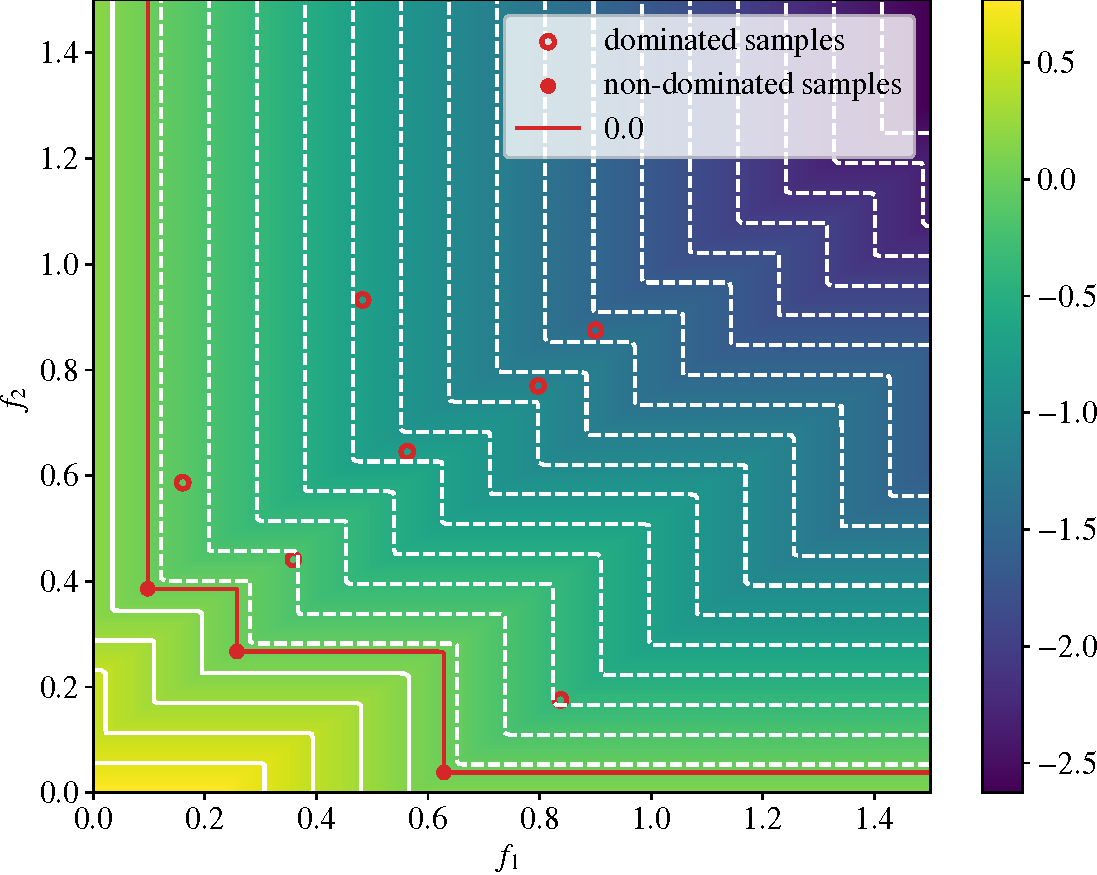
\includegraphics[width=\columnwidth]{figures/_objective_space_SAF_mu.pdf}
    \caption{\safmu}
    \label{fig: saf_obj_space}
\end{subfigure}
\begin{subfigure}[t]{0.45\columnwidth}
    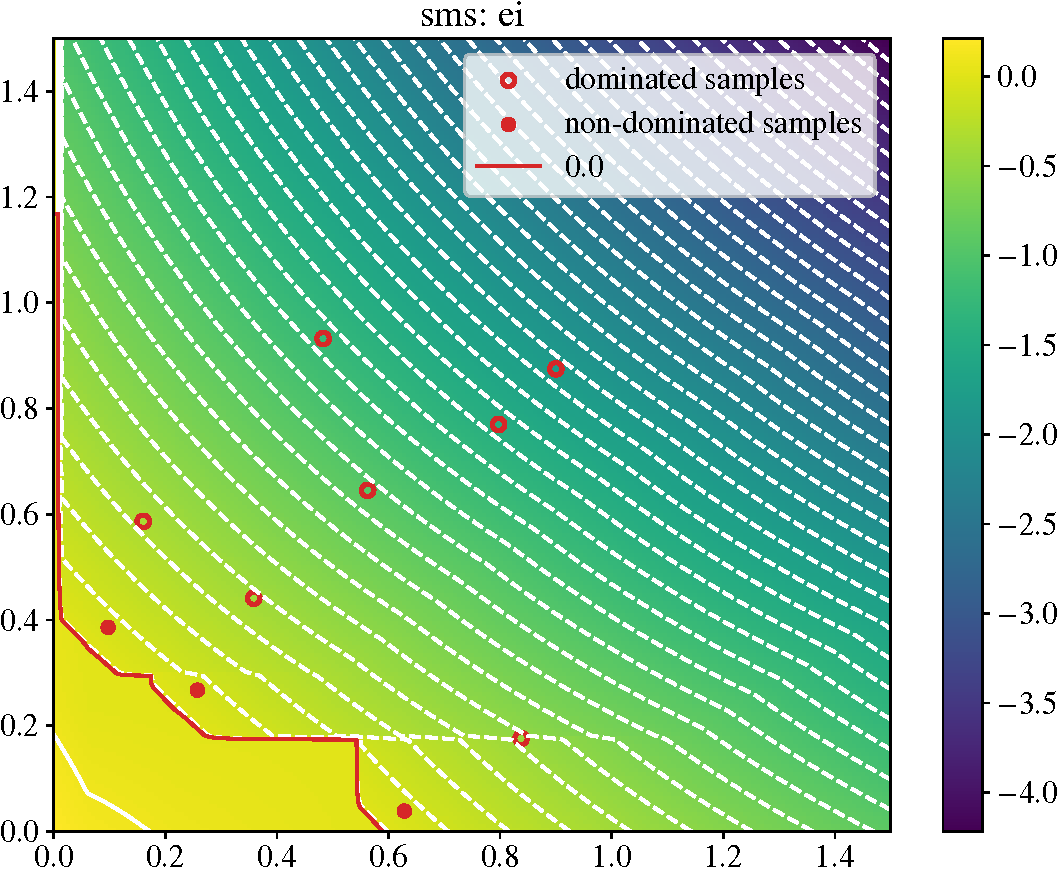
\includegraphics[width=\columnwidth]{figures/_objective_space_SMS_ei.pdf}
    \caption{\smsego}
    \label{fig: smsego_obj_space}
\end{subfigure}
\caption{Visualised infill criteria of a two objective problem, $\nobj=2$. A uniform uncertainly of $\sigma=0.05$ has been applied to the \smsego predictions, with $\epsilon=$ and a reference point for the hypervolume computation of $\rp=1$}
\label{fig: obj_space_comp}
\end{figure}

\begin{algorithm}[t!]
  \SetAlgoLined
  \KwResult{minimiser of $\bff(\mathbf{x})$}
  \SetKwInOut{Input}{Input}
  \SetKwInOut{Output}{output}
  \SetKwComment{tcc}{}{}
  \SetCommentSty{textit}
  \DontPrintSemicolon
  \Input{$\ninitialevaluations$ - number of initial evaluations}
  \Input{$\nbudget$ - evaluation budget}
  \BlankLine
  %\textbf{Initialization}
  %\tcc*[l]{\textbf{Initialisation:}\hfill Generate initial samples}
  $X \gets \text{LHS}(\parameterspace, \ninitialevaluations)$ \label{alg: DSAF_LHS}
  \algremark{Generate initial samples}
  \For {$t = 1 \xrightarrow{} \ninitialevaluations$ \do}{ \label{alg:initial-start_DSAF}
    $\bff_t \gets \bff(\bx_t)$ \algremark{Expensively evaluate initial samples}
  } \label{alg:initial-end_DSAF}
  $\data  \gets \{(\bx_t, \bff_t)\}_{t=1}^{\ninitialevaluations}${\label{alg:inital-evals}}
  \BlankLine
  
 \For{$t = \ninitialevaluations+1\xrightarrow{}\nbudget$ \do}{
 \For{$j=1\xrightarrow{}\nobj$ \do}{
    $\theta_j \gets \text{train} \;\mathcal{GP}(\data)$\algremark{Train GP for each objective \label{alg:train_gp}}
    }
    $\bx_t \gets \underset{\mathbf{x}\in \Omega}{\argmax} \:
    \msafmu(\mathbf{x}, \mathcal{P}, \theta_{1:\nobj})$ \label{alg:opt-alpha_DSAF}
    $\bff_t \gets \bff(\bx_t)$ \label{alg:expensive_DSAF} \algremark{Expensively evaluate $\bx_t$}
    $\data  \gets \data \cup \{(\bx_t, \bff_t )\}$\algremark{Augment data}
 }
 $\{\attainmentset, \attainmentfront\} \gets \data$ \algremark{Select non-dominated evaluations \eqref{eqn: Attainment_set}}
 \Output{$\{\attainmentset, \attainmentfront\}$}
 \caption{\safmu} 
 \label{alg:ourAlg_pseudocde} 
\end{algorithm}


\section{Experimental evaluation}
\subsection{Process}
In this section an analysis is conducted of the performance of \safmu over 150 evaluations of a set of challenging, synthetic MOPs. For comparison we benchmark the state-of-the-art \smsego \cite{ponweiser2008multiobjective} and thec ompetitive, yet computationally efficient \parego \cite{knowles2006parego}. We also compare the, cheap-to-evaluate minimum probability of improvement (\mpoi) infill criteria proposed by Rahat \etal \cite{rahat2017alternative}. For \smsego we formulate the optimiser including the later improvements to the treatment of the objective space dominated by the attainment surface described by Wagner \etal \cite{wagner2010expected}, and the prior knowledge of the objective space required to set the reference point for the hypervolume calculation is assumed to be unknown. Instead the reference point $\rp$ is updated at each evaluation to the maximum value observed in each objective by the current attainment front, plus an offset of $1$, as in the original work $\rp = \max(\attainmentfront)+1$\fnote{I dont think this is clear enough, need to show np.axrgmax($\attainmentfront$, axis=0)}. In order to test the second part of our hypothesis, that more exploitative search will be beneficial, we also include the \ei based \maximin model proposed by Svenson and Santner  \cite{svenson2016multiobjective}, (hereby denoted as \safei), and also a version of \smsego, where the uncertainty from the \gp is ignored, instead using mean prediction only, with no correction for $\epsilon$ (denoted \smsegomu.  

Each optimisation is started from 10 initial \lhs samples, over 31 repeat optimisations of each test function. The repeats are structured so that the same random seed and \lhs samples are used for all optimisation methods within each repeat, and the surrogate used in each of the surrogate methods is an identical \gp applied to the data which has been normalised at each step to have $\mu=0$, $\sigma=1$. Where required the dominated hypervolume is calculated using the Fonseca \etal hypervolume method \cite{fonseca2006improved}.

% \begin{itemize}
    % \item HOW CONDUCTED
    % \item analysis of performance on complex set of problems
    % \item to test two parts of hypothesis we test both mu and ei for saf and sms. And we compare to state of the art, efficient (Parego) and SOA SMS ego. AS well as MPOI method which has been shown to outperform other cheap infills (true?) 
    % \item over budget of 250 evaluations
    % \item 31 repeats of each optimiser
    % \item starting from 10 LHS samples
    % \item paired evaluations
    % \item where required hypervolumes calculated using Fonseca,
    % \item reference points selected from the maximum observed attainment front*1.5
    % \item GPs fitted to data scaled to std 1, mean 0. 
% \end{itemize}

The chosen objective functions for the benchmark tests are a subset the Walking Fish Group problems \cite{huband2005scalable} WFG1-WFG6, which were designed to build on the well-known DTLZ problem set \cite{deb2005scalable} by including deceptive functions and functions where the parameters dictating distance from, and position along the Pareto front are not separable. The dimensionality of the parameter-space $\ndim$ for the WFG problems is scalable, as are the number of objectives $\nobj$. We tested each function over three configurations of each problem in WFG1-WFG6, with 2, 3 and 4 objectives, and parameter spaces ranging from 6-12 dimensions. The exception to this is WFG2, which proved a difficult challenge for all strategies, and so had the parameter space reduced to the minimum permissible $d=[3, 4, 5]$ in order to aid convergence. A full table of the test functions can be seen in Table \ref{tab: f_table}.


\begin{table}[t]
    \setlength{\tabcolsep}{2pt}
    \sisetup{table-format=1.2e-1,table-number-alignment=center}
    \resizebox{0.5\textwidth}{!}{%
        \begin{tabular}{|l|r|l|r|l|}
            \hline
            Function &  $\nobj$ & $\ndim$ & $d$ & Comment\\
            \hline
            WFG1 & 2, 3, 4 & $[0, 2d]^d$ & $3, 4, 5$ &  separable, uni-modal \\
            WFG2 & 2, 3, 4 & $[0, 2d]^d$ & $6, 6, 10$ & non-separable, multi-modal\footnotemark{}, discontinuous Pareto front \\
            WFG3 & 2, 3, 4 & $[0, 2d]^d$ & $6, 10, 10$ &  non-separable, uni-modal \\
            WFG4 & 2, 3, 4 & $[0, 2d]^d$ & $6, 8, 8$ & separable, multi-modal\\
            WFG5 & 2, 3, 4 & $[0, 2d]^d$ & $6, 8, 10$ & separable, deceptive\\
            WFG6 & 2, 3, 4 & $[0, 2d]^d$ & $10, 6, 12$ & non-separable, uni-modal\\
            \hline
        \end{tabular}}
        \caption{Objective functions to be assessed}\label{tab: f_table}
\end{table}
\footnotetext{Multi-modal in only the first objective $f^{1}$, uni-modal in $f^{2} \cdots f^{\nobj}$.}

Two metrics are used to quantify the performance of each optimiser. The first is the dominated hypervolume measure, this is a commonly used means of measuring convergence toward the Pareto front, but as it is also the principal computation behind the $\mathcal{S}$-metric in \smsego. As such we also compare measurements of the Inverted Generational Distance plus (\igd) \cite{ishibuchi2015modified} in order to reduce any unfair advantage to \smsego. $\igdp$ is calculated as:
\begin{equation}
    \igdp(\attainmentfront, \pigdref) = \frac{1}{\abs{\pigdref}}
    \sum_{\mathbf{z}\in\pigdref} \min_{\mathbf{a}\in \attainmentfront} d^{+}(\mathbf{a}, \mathbf{z})
\end{equation}
where $d^{+}$ is the modified Euclidean distance given by:
\begin{equation}
    d^+(\mathbf{z}, \mathbf{a}) = \sqrt{\sum^{\nobj}_{i=1}\max(a_i - z_i, 0)^2}
\end{equation}
Measurements using \igd rely on a set of reference points $\pigdref$ on the problem's Pareto front. In order to ensure no bias toward solutions found in localised regions of this surface it is important that the points be distributed evenly, which is not guaranteed once random samples have been mapped to the Pareto surface with the \textit{Shape Functions} described in the WFG function definitions. In order to achieve an even distribution, we first sample an uneven, but dense population of points on this Pareto front, by evenly sampling the parameter space and applying the aforementioned Shape functions, then calculate a set of evenly distributed points on the attainment surface generated using the methods described by Smith \etal \cite{smith2004dominance}. Attainment surface points which do not lie on the Pareto surface, are then discarded if their nearest neighbour in the set of Pareto optimal points, was greater than a certain threshold. This sampling method was used for all functions with the exception of WFG3, for which the Pareto surface is trivial to compute and sample evenly. The reference points for the ellipsoidal WFG4 with three objectives are shown in Figure \ref{fig: refpoints_wfg4}.  

\begin{figure}[t]
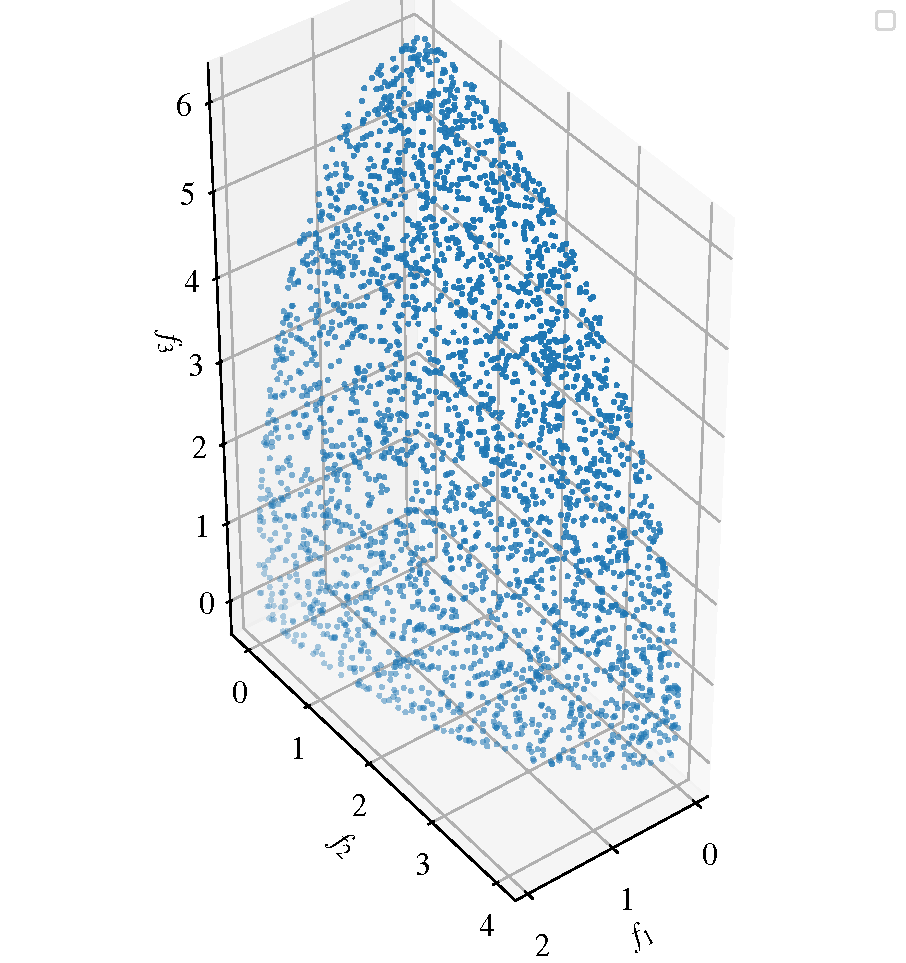
\includegraphics[width=\columnwidth]{figures/_IGD_refpoint_example_WFG4.pdf}
\caption{\igd reference points, for 3 objective WFG4.}
\label{fig: refpoints_wfg4}
\end{figure}

% \begin{itemize}
    % \item HOW ASSESSED
    % \item which problems chosen?
    % \item why problems chosen? build on DTLZ, include various features (multimodal, convex, separable). 
    % \item why d6? reduced dimensionality for wfg1 to facilitate finding better solutions
    % \item measurements taken using dominated hypervolume and igd+
    % \item igd+ samples taken by oversampling the pareto front, and then drawing a random sample from this using the attainment sampling techinique described in richards paper. 
    % \item results compared by their median value, with statistical equivlance tested using Holm-bonferoni corrected wilcoxen signed rank test. 
    % \item problem table
% \end{itemize}

\subsection{Discussion}
The results of the optimisations, as measured by \igd are summarised in table \ref{tab: igd_results}. The performances of the optimisers are, as we may expect, somewhat problem dependant. After the full 150 budgeted evaluations of the objective functions, \safmu either had the lowest median \igd score, or did not differ significantly from the optimiser with the best score in 9 of the 18 tested problems, this is one more than the state-of-the art \smsego, but is equalled by the exploitative adaption \smsegomu. As we might expect, when measured by the $\mathcal{S}$-metric measure the results are somewhat more favourable to \smsego and \smsegomu, with \safmu only being equivalent to the best performer on 9 optimisations, as opposed to \smsegomu's 9. 

Table \ref{tab: igd_results}  however, only considers a slice of the optimisation process, when the algorithms have largely converged. Figure \ref{fig: ranked_plots}\mnote{what are the two different panels showing? why does LHS start at 2 not 1 in the bottom panel?} shows average ranking of each optimiser across all repeats and all problems in the experimental setup, at each step of the optimisation process. Where the difference between optimisations of similar rank have not been statistically significant, as judged by the Wilcoxon signed rank test, the two were assigned the same rank, hence the divergence as the optimisations progress. From this it is clear that \smsegomu performs best in the later stages, whether measuring by \igd or dominated hypervolume, but \safmu is second best by both of these measurement, although performance is similar to \smsego. 

It should be noted that all optimisers performed poorly on WFG2, with the majority of the Pareto Front left unexplored. \parego performed relatively well compared to the other methods, but many of the surrogate models were beaten by the \lhs benchmark here. It is worth noting that WFG2 is the only problem here with a discontinuous Pareto front, and also the only problem in which the boundary between the attainable and unattainable objective space regions, on which the Pareto front lies, extends into the area dominated by the points on the Pareto front. This means much of the objective space, in between the acquired evaluations, and favoured by the infill criteria may unattainable at each step This is a feature which distinguishes this function from the others tested here but could be a factor in the poorer performance by optimisers reliant on infill criteria.\fnote{Not sure this makes sense. We should talk about it and see if you both think it is relevant.} %In all other problems, any point dominated by the current attainment set, is guaranteed to be also attainable. This is not the case for WFG2. 


% \begin{itemize}
%     \item OVERALL
%     % \item As expected performance was problem-specific
%     % \item over the full 150 evaluations SAF-MU was the best performer or equivalent on 7 problems. The same as Sms EI. SMS-Mu was best with 9.
%     % \item For IGD+, saf-mu best on 9. SMS EI best on 8. SMS-MU also best on 9.
%     % % \item this only considers a snapshot of the optimisation process when the optimiser have largely converged. The ranked order can be seen in fig X. "ranks adjusted for equivalence". 
%     % \item WFG1 and 2 converged poorly by infill criteria methods
%     % \item WFG2 converged poorly by all methods
% \end{itemize}

\begin{table}[t]
\begin{subtable}[b]{\columnwidth}
\setlength{\tabcolsep}{2pt}
\sisetup{table-format=1.2e-1,table-number-alignment=center}
\resizebox{\columnwidth}{!}{%
\import{tables/}{igd_table_1.tex}}
\end{subtable}
\begin{subtable}[b]{\columnwidth}
\setlength{\tabcolsep}{2pt}
\sisetup{table-format=1.2e-1,table-number-alignment=center}
\resizebox{\columnwidth}{!}{%
\import{tables/}{igd_table_2.tex}}
\end{subtable}
\begin{subtable}[b]{\columnwidth}
\setlength{\tabcolsep}{2pt}
\sisetup{table-format=1.2e-1,table-number-alignment=center}
\resizebox{\columnwidth}{!}{%
\import{tables/}{igd_table_3.tex}}
\end{subtable}
\caption{\igd results after 150 function evaluations.}
\label{tab: igd_results}
\end{table}

\begin{table}[t]
\begin{subtable}[b]{\columnwidth}
\setlength{\tabcolsep}{2pt}
\sisetup{table-format=1.2e-1,table-number-alignment=center}
\resizebox{\columnwidth}{!}{%
\import{tables/}{hv_table_1.tex}}
\end{subtable}
\begin{subtable}[b]{\columnwidth}
\setlength{\tabcolsep}{2pt}
\sisetup{table-format=1.2e-1,table-number-alignment=center}
\resizebox{\columnwidth}{!}{%
\import{tables/}{hv_table_2.tex}}
\end{subtable}
\begin{subtable}[b]{\columnwidth}
\setlength{\tabcolsep}{2pt}
\sisetup{table-format=1.2e-1,table-number-alignment=center}
\resizebox{\columnwidth}{!}{%
\import{tables/}{hv_table_3.tex}}
\end{subtable}
\caption{Dominated hypervolume results after 150 function evaluations.}
\label{tab: hv_results}
\end{table}

The hypothesis that search based on the mean prediction could offer improvements over \ei approaches appears to be borne out by the results. \smsegomu performs similarly well to \smsego, with few exceptions. There certainly seems to be no advantage to incorporating the uncertainty from the model. This however is not a true \ei method, and does not integrate the posterior prediction to get the expected improvement, but rather calculates the expected improvement to the dominated hypervolume based on the surrogate prediction. \safei is more similar to true \ei, though it uses a Monte-Carlo integration to estimate the model \ei. The performance of \safei is significantly worse than that of \safmu, never once outperforming the mean prediction version. This supports the ideas put forward by De Ath \etal \cite{death2019greed}, that in problems which are complex to model the fortuitous exploration resulting from low surrogate fidelity is sufficient to explore the parameter space.

It appears that broadly speaking \safmu does not surpass the performance of \smsego significantly, but is as good in the majority of cases tested, though the nature of the  function being optimised remains a key factor in which optimiser performs best. 

\begin{figure}[t]
\begin{subfigure}[b]{\columnwidth}
         \centering
         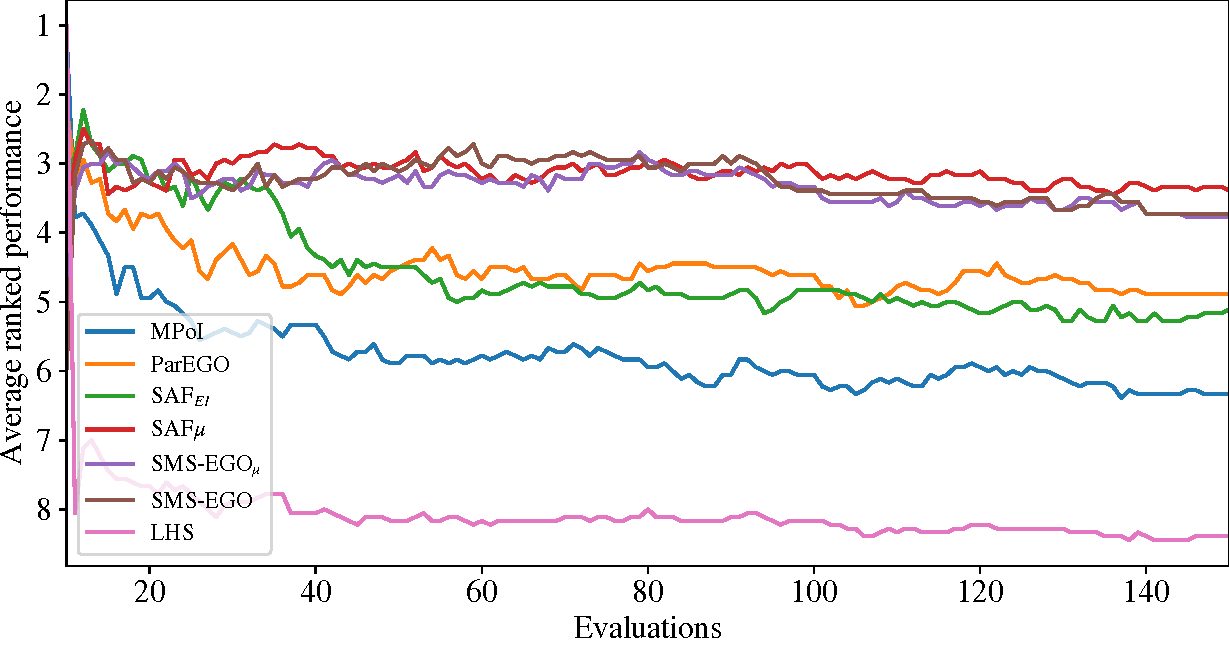
\includegraphics[width=\columnwidth]{figures/_ranked_performance_plot_hv.pdf}
        %  \caption{}
        %  \label{fig: ranked_hv_plot}
     \end{subfigure}
\begin{subfigure}[b]{\columnwidth}
         \centering
         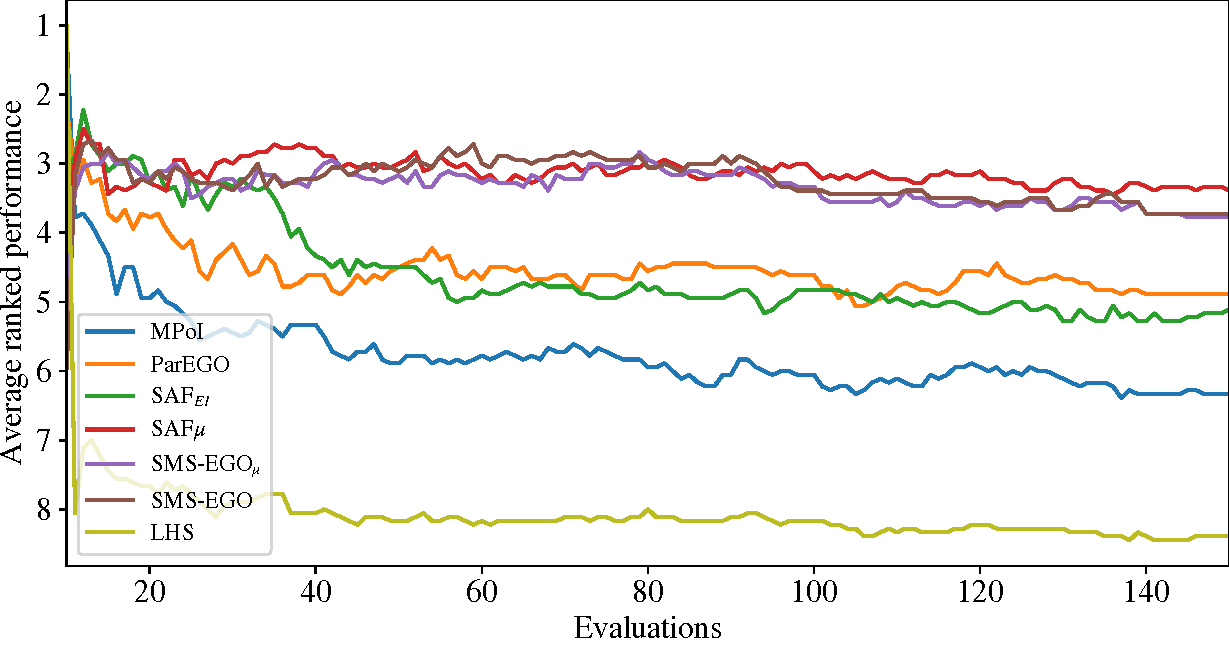
\includegraphics[width=\columnwidth]{figures/_ranked_performance_plot_igd.pdf}
        %  \caption{}
        %  \label{fig: ranked_igf_plot}
     \end{subfigure}
\caption{ranks}
\label{fig: ranked_plots}
\end{figure}

    

\begin{table}[t]
    \setlength{\tabcolsep}{2pt}
    \sisetup{table-format=1.2e-1,table-number-alignment=center}
    \resizebox{0.45\textwidth}{!}{%
    \begin{tabular}{|l|l|l|}
        \hline
        Optimiser name & surrogate  & Comment\\
        \hline
        Saf ei & Multi & \ei version of SAF, as proposed in \cite{svenson2016multiobjective}. \\
        Saf $\mu$ & Multi & Our proposed Optimiser. (See Alg. \ref{alg:ourAlg_pseudocde}) \\
        \smsego: ei & Multi & Current state-of-the-art. \cite{ponweiser2008multiobjective} \\
        \smsego: $\mu$ & Multi & Modification to current SOA to be more exploitative.\\
        ParEgo & Mono & Efficient computation \cite{knowles2006parego}\\
        MPoI & Multi & Benchmark for EMO over infill criteria approach \cite{rahat2017alternative}. \\
        LHS & None & Baseline comparison to pseudo-uniform sampling of parameter space. \\
        \hline
    \end{tabular}}
    \caption{Optimisation strategies to be compared}\label{tab1}
    \label{table:alg_table}
\end{table}


% The WFG problems are intentionally constructed to cover significantly different numerical ranges in the domains of each of their objectives. This presents a problem to the DHV\mnote{has this acronym been defined?} measurement, as the computation of the HV depends heavily on the scales of the objectives. A common solution to this is to optimise a scaled version of the WFG problems where the ranges of each dimension have been normalised, and to set the reference point for the DHV measurement within this scaled objective space, equidistant from the origin. To do this is to assume prior knowledge about the objective function, information which is not typically available in real-world problems. \smsego uses the dominated hypervolume measurement in its process of assessing candidate solutions, and to scale the objectives a priori and provide an ideally positioned reference point is not realistic in a real application. Furthermore setting the DHV reference point for \smsego identically to that against which it is assessed will inevitably give \smsego an unfair advantage, when assessed by the DHV criterion. Instead we will require \smsego to set its own reference point and scale the objectives accordingly. This will be done dynamically during the optimisation in order to normalise the range of each objective present in the non-dominated set of observations. 



\subsection{Conclusion}
When optimising expensive, multi-objective problems efficient use of objective evaluations is critical to convergence within the constraining budget. Current state-of-the-art methods for optimising such problems in few evaluations rely on expensive hypervolume computation which can itself become prohibitively costly as the number of objectives is scaled, and the number of non-dominated solutions in the attainment surface increases. The state-of-the art method is benchmarked on a comprehensive set of synthetic test problems, and an optimisation method based on a cheap, exploitative, \maximin distance infill criteria method from the attainment surface is presented and shown to be similarly effective across the test problems. The leading efficient methods are also tested, and surpassed in the majority of tested functions by our proposed approach. 

Benchmarking on the same set of problems we further show that approaches which leverage the uncertainty in the surrogate posterior prediction offer no improvement over simple mean prediction when it comes to complex EMO problems, and in the majority of cases, optimisations which use pure mean prediction are more effective. This expands the scope of effective surrogate models for efficient Bayesian Optimisation style surrogate approaches to MOP's, to methods which may be better able to model mean prediction but do not provide the posterior uncertainty estimates that come with A \gp surrogate.

% \section{Definitions required}
% \begin{enumerate}
%     \item Objective space
%     \item Domination
% \end{enumerate}


% \section{Consideratios/ammendments to be made}
% \begin{itemize}
%     \item hyphenate multisurrogate, monosurrogate, single surrogate
%     \item check for consistency in parameters vs inputs, 
%     \item Do i need to explain traingp in algorithms?
%     \item MOOP vs MOP vs MOO<- pick one
%     \item define HV
%     \item state of the art vs state-of-the-art
%     \item check  S-metric
% \end{itemize}
\bibliographystyle{ieeetr}
\bibliography{bibliography}

\end{document}

%%% Local Variables:
%%% mode: latex
%%% TeX-master: t
%%% End:

